\chapter{Introduzione al Deep Learning}

La prima cosa che vogliamo sia ben chiara è la differenza fra Machine Learning e Deep Learning. Per far ciò bisogna partire dall'analizzare ciò che facevamo con i programmi di Machine Learning, riferendoci a uno specifico caso d'uso. Partiamo considerando il caso d'uso del riconoscimento d'immagine, quello che effettivamente risulta più semplice come esempio da prendere in analisi, successivamente comprendiamo quali sono le differenze con un modello di Deep Learning. Noi solitamente partivamo dal creare un programma, questo programma doveva essere in grado, data un'immagine, di estrarre alcuni attributi per poi utilizzarli all'interno di un modello di ML e riuscire a riconoscere immagini della stessa tipologia. Il passo ulteriore che viene effettuato dal Deep Learning è un passaggio effettuato a monte, ossia durante la selezione degli attributi, noi costruiamo una vera e propria gerarchia degli attributi, avendo la possibilità di stabilire attributi di basso livello, medio livello e alto livello. Questa selezione degli attributi viene effettuata da dei modelli di Machine Learning, creando nella sua complessità un meccanismo automatico più raffinato.

\begin{figure}
    \centering
    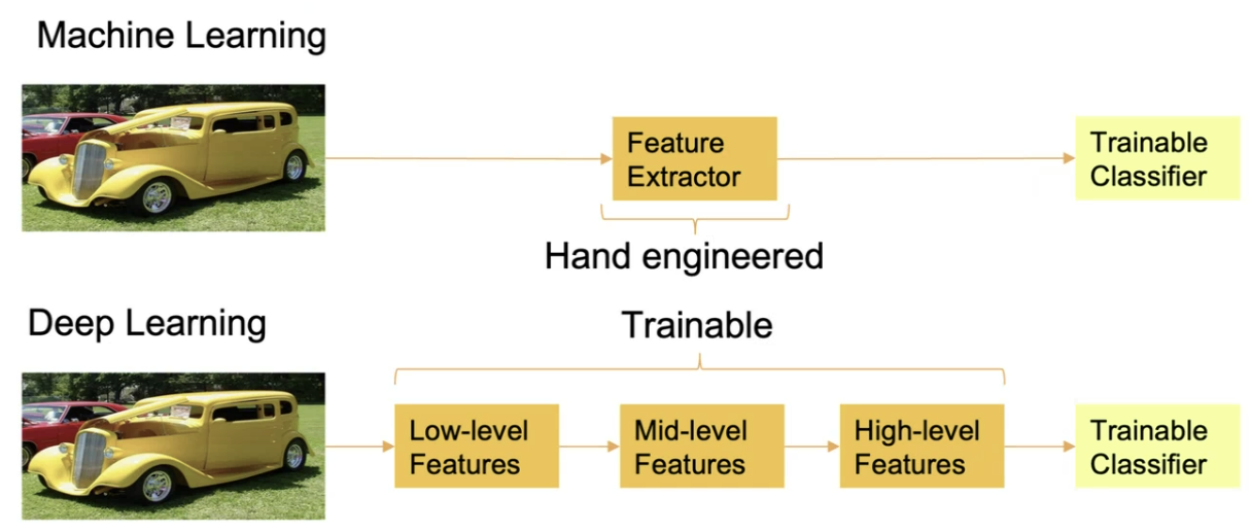
\includegraphics[width=0.75\linewidth]{figure/DeepMachineDiff.png}
    \caption{Schema che rappresenta la principale differenza fra un modello di Machine Learning e di Deep Learning}
    \label{fig:DLMLDiff}
\end{figure}

\section{Definizione}
Il Deep Learning è una sotto-disciplina del Machine Learning la quale utilizza reti neurali profonde, dunque delle reti neurali con numerosi hidden-layer, per poter estrarre delle rappresentazioni gerarchiche dai dati. A differenza dei metodi tradizionali di Machine Learning, i quali richiedono l'ingegnerizzazione manuale delle caratteristiche, il Deep Learning è in grado di apprendere automaticamente rappresentazioni multi-livello, direttamente dai dati grezzi. Questo approccio, si è dimostrato particolarmente efficace in campi come la visione artificiale, il riconoscimento vocale e l'elaborazione del linguaggio naturale.

\section{Esempio: Il dataset MNIST}
MNIST è un dataset ampiamente utilizzato per il riconoscimento di cifre scritte a mano. È composto da 60.000 immagini di addestramento e 10.000 immagini di test, ognuna delle quali è una griglia 28x28 di pixel in scala di grigi. L'obiettivo di un modello di apprendimento automatico addestrato su MNIST è quello di classificare correttamente ogni immagine in una delle 10 categorie (da 0 a 9). Questo dataset è spesso utilizzato come benchmark per valutare le prestazioni di nuovi algoritmi di apprendimento profondo.
\\
\begin{figure}[h]
    \centering
    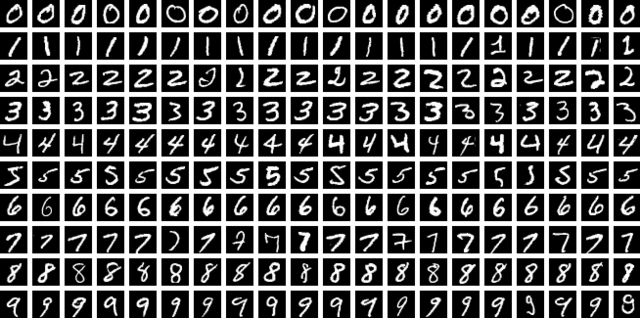
\includegraphics[width=0.75\textwidth]{figure/MNIST_dataset_example.png}
    \caption{Rappresentazione di un esempio delle immagini presenti nel dataset del MNIST.}
\end{figure}

\section{Grafi Computazionali}
Un Grafo computazionale (Figura~\ref{fig:computationalG}) rappresenta il flusso di operazioni tra variabili, esso viene utilizzato per modellare i calcoli effettuati in una rete neurale. Ogni nodo del grafo rappresenta un'operazione matematica, mentre i bordi o archi, rappresentano i flussi di dati con le loro informazioni. Utilizzando questa struttura, possiamo visualizzare e ottimizzare il flusso di informazioni e il processo di apprendimento della rete. Ad esempio, in una rete neurale profonda, ogni livello applica una trasformazione ai dati, tramite l'utilizzo di una funzione di attivazione, generando un input il quale verrà poi propagato fino al livello finale, per ottenere una previsione. Come possiamo osservare nella figura con il blocco relativo alla \textbf{regressione logistica}. Il modello utilizzato da noi, invece, distingue nettamente i vari elementi tramite l'utilizzo di forme e colori, in modo da essere maggiormente intuitivo, avendo una differenza fra input, funzioni deterministiche e funzioni scalari (Figura~\ref{fig:parModel}).

\begin{figure}
    \centering
    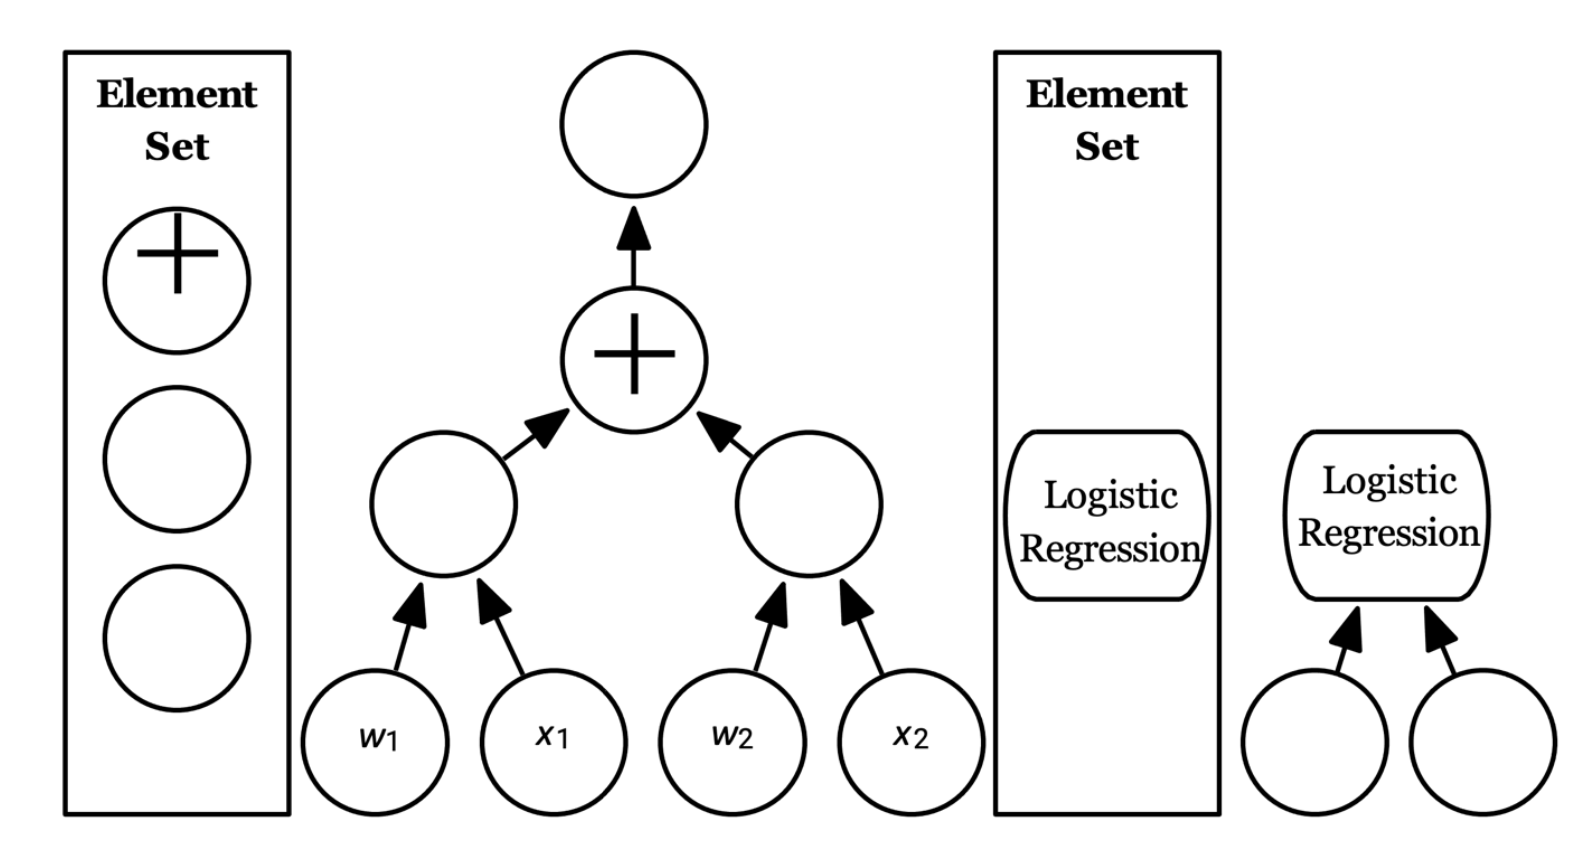
\includegraphics[width=0.75\linewidth]{figure/ComputationalGraph.png}
    \caption{Rappresentazione di un grafo computazionale, i quali vari elementi vengono rappresentati da forme differenti.}
    \label{fig:computationalG}
\end{figure}
\begin{figure}
    \centering
    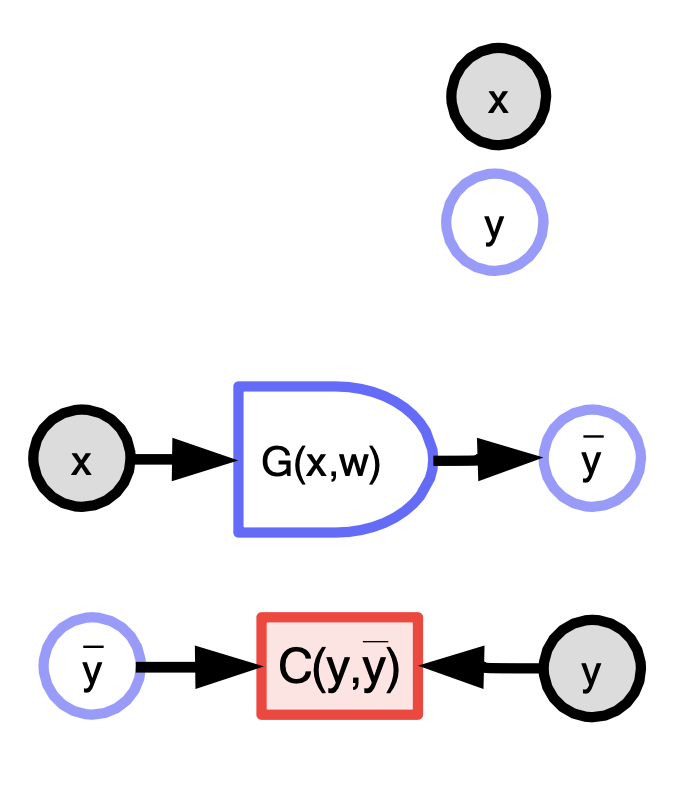
\includegraphics[width=0.40\linewidth]{figure/ParametriModel.png}
    \caption{Notazione dei nostri modelli, dall'alto verso il basso ci sono: Variabili, Funzione deterministica e Funzione scalare}
    \label{fig:parModel}
\end{figure}

\section{Funzione di costo}
Una \textbf{funzione di costo} è un esempio di calcolo riportabile tramite l'utilizzo dei nostri grafi computazionali (Figura~\ref{fig:costFunction}). Questa funzione misura l'errore tra l'output del modello e l'output desiderato, ed è fondamentale per il processo di apprendimento. Il modello infatti, cerca di minimizzare questa funzione aggiustando i pesi della rete attraverso l'algoritmo di ottimizzazione. Una delle funzioni di costo più comuni nel contesto delle reti neurali è l'errore quadratico medio (MSE), definito come:
\begin{equation}
    C(y, \hat{y}) = \frac{1}{n} \sum_{i=1}^{n} (y_i - \hat{y}_i)^2
\end{equation}
Dove $y_i$ rappresenta il valore reale e $\hat{y}_i$ l'output predetto dal modello per il campione $i$-esimo. Minore sarà il valore della funzione di costo, migliore sarà la capacità del modello di effettuare previsioni accurate.

\begin{figure}
    \centering
    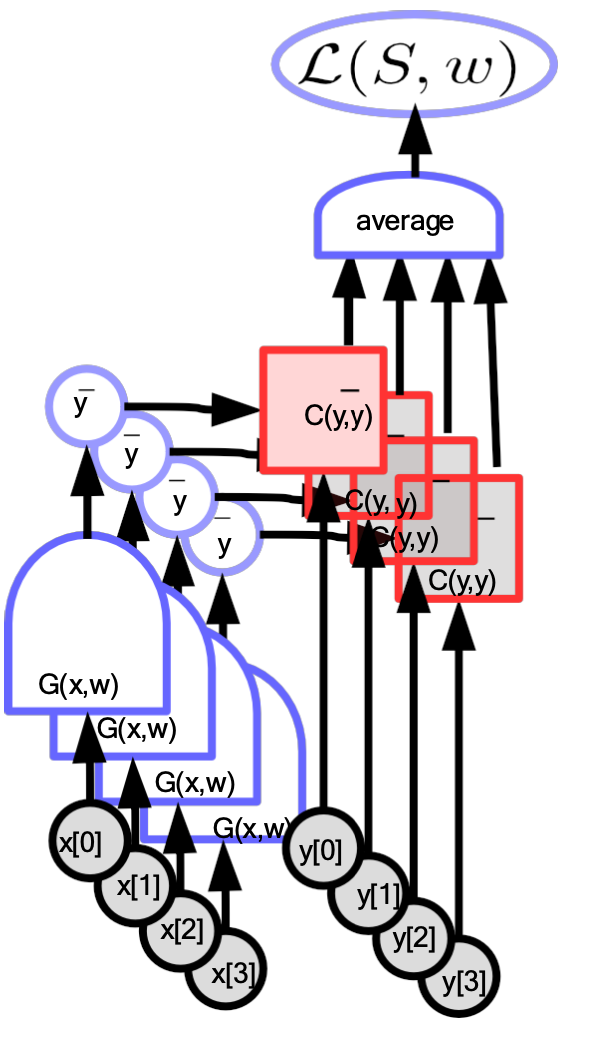
\includegraphics[width=0.30\linewidth]{figure/CostFunction.png}
    \caption{Rappresentazione tramite l'utilizzo di un grafico computazionale della funzione di costo, utilizzando il MSE}
    \label{fig:costFunction}
\end{figure}

\section{Reti Neurali}
Una Rete Neurale è una pila di blocchi funzionali lineari e non lineari, le quali entità fondamentali prendono il nome di neuroni(Figura~\ref{fig:neuralNet}). Ogni \textbf{neurone} calcola una somma pesata degli input ricevuti e applica una funzione di attivazione per introdurre non linearità nel modello. Questa architettura permette alla rete di apprendere rappresentazioni complesse dei dati. Un singolo neurone in una rete neurale può essere rappresentato come:
\begin{equation}
    z = \sum_{i=1}^{n} w_i x_i + b
\end{equation}
Dove $w_i$ sono i pesi associati agli input $x_i$, e relativi al bias $b$. Successivamente, viene applicata una funzione di attivazione $\sigma(z)$ in modo tale da ottenere un output finale:
\begin{equation}
    y = \sigma(z)
\end{equation}

Le reti neurali, non sono altro che strutture complesse composte da questi neuroni, i quali possono essere completamente collegati fra loro, generando le \textit{Fully-Connected Neural Network}, oppure collegate parzialemente creandone di diversa tipologia, questi neuroni vengono concatenati formando diversi strati, formando delle archittetture profonde, ossia composte da diversi strati.

\begin{figure}[h]
    \centering
    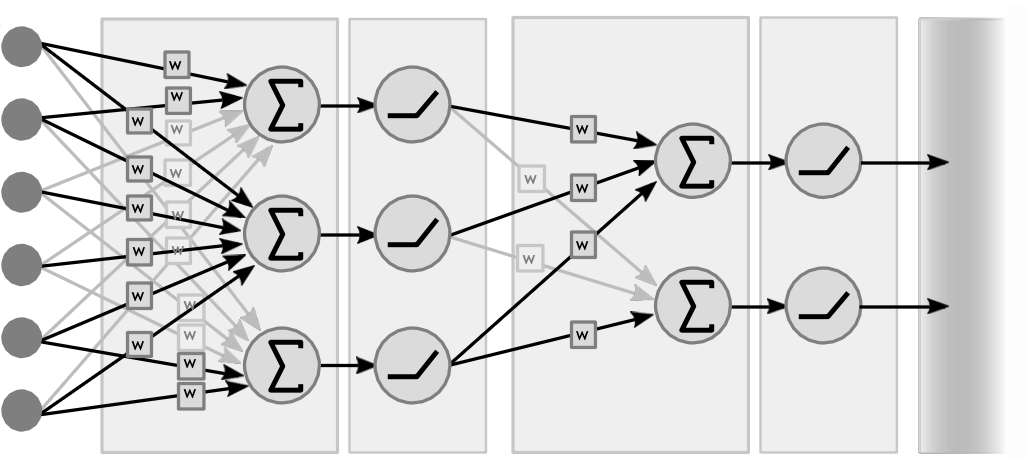
\includegraphics[width=0.85\textwidth]{figure/NeuralNet.png}
    \caption{Figura rappresentativa di un esempio di rete neurale con diversi strati nella sua architettura.}
    \label{fig:neuralNet}
\end{figure}

\section{Backpropagation}
La \textbf{Backpropagation} (retropropagazione), è uno degli algoritmi fondamentali nel momento in cui si parla di reti neurali, poiché permette di allenare la rete, basandosi sulla \textbf{discesa del gradiente}. L'idea fondamentale della Backpropagation, è propagare all'indietro l'errore generato dalla predizione e dal valore effettivo, in modo tale da aggiornare i pesi della rete, affinché venga ridotto l'errore complessivo (ossia la funzione di perdita o loss function). Il processo di Backpropagation consente di calcolare i gradienti dell'errore, rispetto ai pesi della rete e poter propagare questi gradienti attraverso la rete all'indietro, in modo tale da aggiornare i pesi e ottenere dei risultati sempre più accurati di volta in volta fintantoché non si raggiunge a una convergenza dei valori dei pesi.

\subsection{Calcolo dei Gradienti}
Il cuore della Backpropagation risiede nel calcolo dei gradienti della funzione di perdita rispetto ai pesi, utilizzando la \textbf{regola della catena}.
\begin{Definizione}
    La regola della catena afferma che se $f(x)$ e $g(x)$ sono funzioni derivabili, allora la derivata della funzione composta $h(x) = f(g(x))$ è:
    \[
    \frac{\partial h}{\partial x} = \frac{\partial f}{\partial g} \cdot \frac{\partial g}{\partial x}
    \]
\end{Definizione}
\marginpar{\href{https://cannydatascience.medium.com/backpropagation-come-apprende-una-rete-neurale-91c0c900fbc}{Approfondimento sulla Backpropagation}}
L'algoritmo di Backpropagation calcola i gradienti da ogni layer e li propaga all'indietro, aggiornando i pesi della rete. Il gradiente indica la direzione nella quale i pesi devono essere aggiornati per ridurre l'errore complessivo. La formula generale per la derivata della funzione di costo rispetto ai pesi è la seguente:
\begin{equation}
    \frac{\partial C}{\partial W} = \frac{\partial C}{\partial y} \cdot \frac{\partial y}{\partial W}
\end{equation}
Dove $C$ rappresenta la funzione di costo, $y$ l'output del modello e $W$ il peso da aggiornare. Questo processo viene ripetuto per ogni livello della rete, fino a che i pesi non convergono verso valori ottimali. Questa procedura può essere facilmente sintetizzata in maniera più dettagliata in un grafo computazionale (Figura~\ref{fig:backPropGraph}), ovviamente entrando più nel dettaglio e analizzando i calcoli come abbiamo già visto nel corso di Machine Learning. Nell'algoritmo della backpropagation è possibile applicare qualunque grafo che sia diretto e aciclico. Nel caso in cui il grafo presentasse dei loop, sarà necessario scioglierli.

\begin{figure}
    \centering
    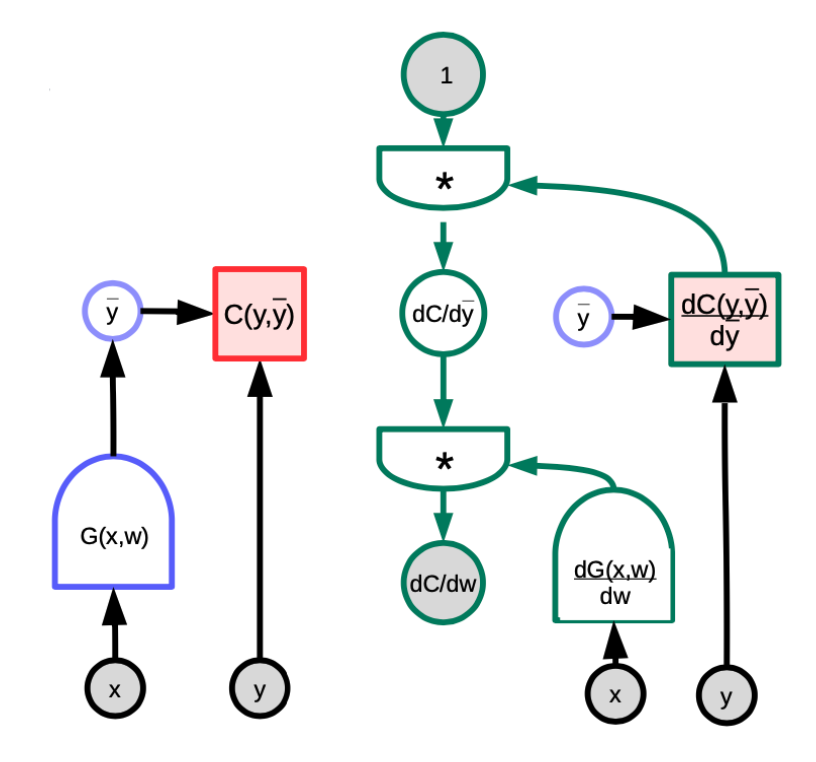
\includegraphics[width=0.5\linewidth]{figure/BackPropGraph.png}
    \caption{Grafo computazionale della Backpropagation, che si integra con quello già precedentemente visto della funzione di costo in modo tale da raffinare gli esiti finali correggendosi dinamicamente}
    \label{fig:backPropGraph}
\end{figure}

\section{Problemi della Backpropagation}
Uno dei principali problemi della Backpropagation nel campo del Machine Learning è il \textit{problema del gradiente che scompare o esplode}. Questo problema si verifica quando il gradiente della funzione di costo rispetto ai pesi diventa molto piccolo o molto grande nei livelli più profondi della rete.

\begin{itemize}
    \item \textbf{Gradiente che scompare}: nelle reti molto profonde, i gradienti calcolati per i livelli iniziali diventano sempre più piccoli man mano che vengono propagati all'indietro. Questo porta a aggiornamenti minimi dei pesi nei primi livelli, rallentando drasticamente l'addestramento o impedendo alla rete di apprendere.
    \item \textbf{Gradiente che esplode}: al contrario, se i gradienti aumentano esponenzialmente durante la propagazione all'indietro, i pesi della rete possono diventare estremamente grandi, portando a instabilità nell'addestramento e rendendo difficile la convergenza.
\end{itemize}

Grazie all'avanzamento della ricerca il Machine Learning si è evoluto in Deep Learning, sviluppando diverse soluzioni, affinché queste problematiche venissero mitigate:

\begin{enumerate}
    \item \textbf{Funzioni di attivazione avanzate}: L'utilizzo di \textbf{ReLU} (Rectified Linear Unit) ha ridotto il problema del gradiente che scompare rispetto a sigmoid e tanh. Varianti come Leaky ReLU e Parametric ReLU migliorano ulteriormente l'apprendimento;
    \item \textbf{Inizializzazione dei pesi}: Metodi di inizializzazione dei pesi come \textbf{Xavier} per l'assegnamento dei pesi stabilizzano i gradienti all'inizio dell'addestramento;
    \item \textbf{Batch Normalization}: Tecnica la quale permette di normalizzare le attivazioni intermedie riducendo la varianza dei gradienti durante la propagazione.
\end{enumerate}

L'introduzione infatti di queste tecniche, ma anche l'introduzione di altre, hanno permesso al Deep Learning di diventare un campo di studio sempre più interessante, divenendo anche più efficace come tecnica rispetto all'utilizzo di metodi tradizionali postulati dal Machine Learning.

\section{Implementazione con PyTorch}
Giusto per effettuare una parallelizzazione della teoria, con l'aspetto implementativo del Deep Learning, quì mostriamo come implementare una rete neurale utilizzando \textbf{PyTorch}, per far ciò possiamo utilizzare la classe \texttt{nn.Module} in modo tale da definire la nostra architettura. Di seguito un esempio di una semplice rete con due livelli nascosti:
\\
\begin{python}[frame=trBL]
    import torch
    from torch import nn

    class MyNet(nn.Module):
        def __init__(self, input_dim, hidden_dim, output_dim):
            super().__init__()
            self.fc1 = nn.Linear(input_dim, hidden_dim)
            self.fc2 = nn.Linear(hidden_dim, output_dim)
    
        def forward(self, x):
            x = torch.relu(self.fc1(x))
            x = self.fc2(x)
            return x
    model = MyNet(784, 128, 10)
\end{python}
\vspace{0.5em}
La rete in questo codice prende in input delle immagini di 28x28 pixel (convertite in vettori di 784 elementi), le elabora utilizzando un livello nascosto con 128 neuroni e produce infine un output di 10 neuroni corrispondenti alle 10 classi del dataset MNIST.